\begin{minipage}{0.63\linewidth}
    On considère deux aimants droits $A_1$ et $A_2$ créant chacun en $P$ des champs
    magnétiques notés respectivement $\vec{B}_1$ et
    $\vec{B}_2$. Leurs valeurs sont $\vec{B}_1=\qty{30}{\mT}$ et
    $\vec{B}_2=\qty{40}{\mT}$. Les axes des deux aimants sont perpendiculaires.
    \begin{enumerate}
        \item Compléter le schéma en indiquant les pôles des aimants.
        \item Construire graphiquement en $M$ le champ magnétique $\vec{B}$
              résultant de la superposition de $\vec{B}_1$ et $\vec{B}_2$.
        \item Calculer l'intensité $B$.
        \item Dessiner l'orientation d'une aiguille aimantée qu'on placerait au
              point $M$.
        \item Calculer l'angle $\alpha=\left(\widehat{\vec{B}_2,\vec{B}}\right)$.
    \end{enumerate}
\end{minipage}
\hfill
\begin{minipage}{0.35\linewidth}
    \flushright
    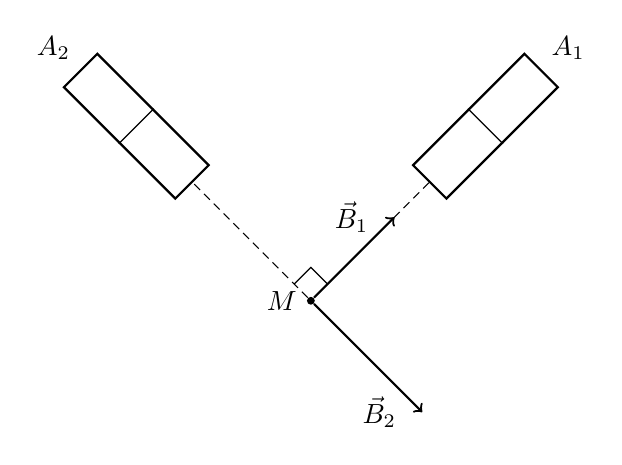
\begin{tikzpicture}
        \foreach \x/\a [count=\i] in {1/-45,-1/45}{%
        \node[inner sep=0pt,draw,thick,minimum width=6mm,minimum height=2cm,
            rotate=\a,anchor=south,label=$A_{\i}$] (A\i) at (\x*1.5,1.5) {};
        \draw (A\i.east) -- (A\i.west);
        }
        \node[circle,inner sep=1pt,fill,label=left:$M$] (M) at (0,0) {};
        \draw[densely dashed] (A1.south) -- (M) -- (A2.south);
        \draw[->,thick] (M) -- ++(45:1.5) node[left=2mm] {$\vec{B}_{1}$};
        \draw[->,thick] (M) -- ++(-45:2) node[left=2mm] {$\vec{B}_{2}$};
        \draw ([shift=(135:0.3)]M.center) -- ++(45:0.3) -- ++(-45:0.3);
    \end{tikzpicture}
\end{minipage}

